\documentclass[iop,apj]{emulateapj}
\usepackage{amsmath,amssymb,amstext}

%\usepackage[breaklinks,colorlinks,citecolor=blue,linkcolor=magenta]{hyperref} 
%\renewcommand*{\sectionautorefname}{Section}
%\usepackage[all]{hypcap} %Links go to figures; breaks on deluxetables (use \capstartfalse \capstarttrue to fix it)

\usepackage{aas_macros}
\usepackage{natbib}
%\usepackage{siunitx}
\bibliographystyle{apj}

\shorttitle{Short Title}
\shortauthors{Author et al.}




\newlength{\colwidth}\setlength{\colwidth}{3.5in}

\addtolength\voffset{0.8cm}

\newcommand{\ds}{\displaystyle}
\newcommand{\be}{\begin{equation}}
\newcommand{\ee}{\end{equation}}
\newcommand{\bee}{\begin{eqnarray}}
\newcommand{\eee}{\end{eqnarray}}

\newcommand{\ov}{ \Omega_{\rm \Lambda} }
\newcommand{\om}{ \Omega_{\rm m} }
\newcommand{\mob}{ M_{\rm obj} }
\newcommand{\mstar}{ M_{*}(a) }
\newcommand{\msol}{\hbox{${\rm M}_\odot$}}

\newcommand{\rvir}{\hbox{$r_{\rm 200}$}}
\newcommand{\mvir}{\hbox{$M_{\rm vir}$}}
\newcommand{\Mvir}{\hbox{$M_{\rm vir}$}}
\newcommand{\vvir}{\hbox{$v_{\rm 200}$}}
\newcommand{\tvir}{T_{\rm vir}}
\newcommand{\mthresh}{M_{\rm t}}
\newcommand{\nsats}{n_{\rm sats}}
\newcommand{\vmax}{{\rm v}_{\rm max}}
\newcommand{\zreion}{z_{\rm reion}}
\newcommand{\LCDM}{$\Lambda$CDM }
\newcommand{\sigate}{ \sigma_{8}}
\newcommand{\actoy}{a_{c,{\rm toy}}}
\newcommand{\K}{{\rm K}}

\newcommand{\DME}{D_{\rm M31}}
\newcommand{\vMEI}{v_{\rm M31}}
\newcommand{\MMEI}{M_{\rm M31}}
\newcommand{\DMEE}{D_{\rm M33}}
\newcommand{\vMEE}{v_{\rm M33}}
\newcommand{\MMEE}{M_{\rm M33}}
\newcommand{\MMW}{{\rm M}_{\rm MW}}
\newcommand{\Nsubs}{N_{\rm subs}}

\def\rx{X}
\def\ry{Y}
\def\rz{Z}
\def\vx{v_X}
\def\vy{v_Y}
\def\vz{v_Z}
\def\distance{D}
\def\vrad{v_{\rm rad}}
\def\vtan{v_{\rm tan}}

\def\pr{{\rm Pr}}
\def\pars{\mathbf{x}}
\def\parsi{x_i}
\def\data{\mathbf{d}}
\def\datai{d_i}
\def\datap{\mathbf{d}^{\rm p}(\pars)}
\def\datapi{d^{\rm p}_{i}(\pars)}

\newcommand{\Msun}{{\rm M}_\odot}
\newcommand{\hinv}{h^{-1}}
\newcommand{\Mpc}{{\rm Mpc}}
\newcommand{\hmpc}{\hinv\Mpc}
\newcommand{\kpc}{{\rm kpc}}
\newcommand{\kms}{{\rm km s}^{-1}}

\newcommand{\rhobar}{\langle \rho \rangle}
\newcommand{\sig}{ \langle \sigma v \rangle }
\newcommand{\sigwig}{ {\widetilde \sigma} }
\newcommand{\rbh}{ r_{\rm bh} }
\newcommand{\rmax}{ r_{\rm max} }
\newcommand{\kmsmpc}{\, \rm{km}\,  \rm{s}^{-1}\, \rm{Mpc}^{-1}}
\newcommand{\lsim}{\lower.5ex\hbox{\ltsima}}
\newcommand{\gsim}{\lower.5ex\hbox{\gtsima}}
\newcommand{\ltsima}{$\; \buildrel < \over \sim \;$}
\newcommand{\gtsima}{$\; \buildrel > \over \sim \;$}
\def \etal      {\hbox{et al.} }

\newcommand{\bolshoi}{{\sc Bolshoi }}
\newcommand{\consuelo}{{\sc Consuelo }}
\newcommand{\subfind}{\texttt{\footnotesize SUBFIND }}
\newcommand{\CMBFAST}{\texttt{\footnotesize CMBFAST }}

\def\Sref#1{Section~\ref{#1}}
\def\Fref#1{Figure~\ref{#1}}
\def\Tref#1{Table~\ref{#1}}
\def\Eref#1{Equation~\ref{#1}}
\def\Aref#1{Appendix~\ref{#1}}

%%%%%%%%%%%%%%%%%%%%%%%%%%%%%%%%%%%%%%%%%
% RESULTS:

\def\MLG{M_{\rm LG}}
\def\MMW{M_{\rm MW}}
\def\MEI{M_{\rm M31}}
\def\MEE{M_{\rm M33}}

% Local group mass: MW+M31 from M31 kinematics:
\def\MPAIRestimate{XX}
\def\MPAIRerrorplus{xx}
\def\MPAIRerrorminus{xx}

% Local group timing argument quantities:
\def\ATA{A_{200}}
\def\MTA{M_{LG,TA}}

% Mass of M31+M33 system, from M33 kinematics:
\def\MbAestimate{XX}
\def\MbAerrorplus{xx}
\def\MbAerrorminus{xx}

% Mass of local group, MW+M31, from both M31 and M33 kinematics:
\def\MTRIPLETestimate{XX}
\def\MTRIPLETerrorplus{xx}
\def\MTRIPLETerrorminus{xxx}

% Individual galaxyhalo mass estimates from both M31 and M33 kinematics:
\def\MEIestimate{XX}
\def\MEIerrorplus{xx}
\def\MEIerrorminus{xx}

\def\MEEestimate{XX}
\def\MEEerrorplus{xx}
\def\MEEerrorminus{xx}

\def\MMWestimate{XX}
\def\MMWerrorplus{xx}
\def\MMWerrorminus{xx}

%%%%%%%%%%%%%%%%%%%%%%%%%%%%%%%%%%%%%%%%%

\usepackage[usenames]{color}
\newcommand{\risa}[1]{\textcolor{red}{\bf #1}}
\newcommand{\phil}[1]{\textcolor{ForestGreen}{\bf #1}}
\newcommand{\mike}[1]{\textcolor{Violet}{\bf #1}}
\newcommand{\question}[1]{\textcolor{blue}{\bf #1}}
\newcommand{\todo}[2]{{\bf To do (#1): #2}}
\newcommand{\new}[1]{{\bf #1}}

\newenvironment{inlinefigure}{\def\@captype{figure}

\noindent\begin{minipage}{0.999\linewidth}\begin{center}}
{\end{center}\end{minipage}\smallskip}

\citestyle{aa}
\shortauthors{Williamson et al.}
\shorttitle{The Mass of the Local Group}

% ----------------------------------------------------------------------------

\begin{document}

\title{The Dark Matter Distribution of the Local Group inferred from
Cosmological Simulations: I. The Halo Masses of M31, M33 and the Milky Way}


\author{Marc Williamson\altaffilmark{1}}
\author{Philip J. Marshall\altaffilmark{1}}
\author{Michael T. Busha\altaffilmark{2}} 
\author{Risa H. Wechsler\altaffilmark{1}}

\altaffiltext{1}{Kavli Institute for Particle Astrophysics and Cosmology, Stanford, CA, 94305, USA
{\tt mwillia1@stanford.edu, pjm@slac.stanford.edu, rwechsler@stanford.edu}}
\altaffiltext{2}{???}


% ----------------------------------------------------------------------------

\begin{abstract} 

We study the local group of galaxies by identifying analogous systems in the \consuelo N-body simulation.  The \consuelo halo catalogs are treated as a large sample drawn from the cosmological prior PDF, and local group analogs are identified by matching the observed kinematics of the system.  Weights are calculated for the \consuelo sample by finding the likelihoods for the simulated kinematic properties compared to observations.  We study the effect of including the existence and kinematics of M33 on the posterior distributions of the local group mass by using three types of samples: from only the "observed" galactocentric distance, radial velocity, and tangential velocity of M31, we infer the mass of the local group to be $\MLG =
(\MMW + \MEI) = (\MPAIRestimate^{+\MPAIRerrorplus}_{-\MPAIRerrorminus}) \times
10^{12} \Msun$. Including the only the existence of M33 as a condition for identifying local group analogs results in a different inference of the mass, $\MLG =
(\MMW + \MEI) = (\MPAIRestimate^{+\MPAIRerrorplus}_{-\MPAIRerrorminus}) \times
10^{12} \Msun$. Finally including the kinematics of M33 we infer the mass of the local group to be $\MLG =
(\MMW + \MEI) = (\MPAIRestimate^{+\MPAIRerrorplus}_{-\MPAIRerrorminus}) \times
10^{12} \Msun$.  This is ... than the mass that has been estimated from the
timing argument: we show that for our matched analogs the timing argument mass
systematically ... the local group mass.  We are also able to estimate the halo masses of the three galaxies
individually, finding these to be $\MEI =
(\MEIestimate^{+\MEIerrorplus}_{-\MEIerrorminus}) \times 10^{12} \Msun$, $\MEE
= (\MEEestimate^{+\MEEerrorplus}_{-\MEEerrorminus}) \times 10^{12} \Msun$, 
and $\MMW = (\MMWestimate^{+\MMWerrorplus}_{-\MMWerrorminus}) \times 10^{12}
\Msun$. 
%
This Milky Way halo mass estimate is in xxxagreement with previous estimates
from stellar and dwarf satellite kinematics.


\end{abstract}

\keywords{%
Galaxy: halo, fundamental parameters -- 
galaxies: haloes, fundamental parameters -- 
galaxies: Local Group -- 
galaxies: individual: M31, M33 --
cosmology: dark matter}

% ----------------------------------------------------------------------------

\section{Introduction}
\label{sec:intro}

The Local Group (LG) of galaxies consists of two large spiral galaxies,
Andromeda (M31) and the Milky Way (MW), and a population of smaller
satellite galaxies, the biggest of which is Triangulum (M33). We know
relatively little about the distribution of dark matter throughout the Local
Group volume, beyond simple estimates of the total mass of the group
estimated from its members kinematics \citep[e.g.\ ][hereafter VG08]{vdM+G08}.
Our knowledge of the dark matter halos of the group member galaxies is
similarly sparse: virial masses have been estimated from extrapolations of
simple models fitted to stellar or gas kinematics \citep[e.g.\
][]{Xue+08,M31rotcurve} or to the observed positions and 
velocities of satellite galaxies \citep[e.g.\ ][]{EvansEtc}. 

Our goal is to tightly constrain the mass of the Local Group
by combining observational data on the  positions and velocities of the
three largest LG members with our understanding of structure formation
in $\Lambda$CDM universes, as detailed in halo catalogs extracted from
cosmological N-body simulations. We treat halo catalogs as containing
samples drawn from a very informative, highly correlated prior PDF for
halo properties, and then  calculate weighted posterior PDF's using likelihood
functions based on the observed kinematics of the particular system
under study. In \citet[][hereafter B11]{Bus++11} we presented a new
measurement of the Milky Way halo mass, made in this way using the
\bolshoi simulation of \citet{Bolshoi} and the distances to and speeds
of the Magellanic Clouds. In this work, we use the lower resolution but
higher volume \consuelo simulations, and constrain them with the radial
velocities, proper motions and distances of M31 and M33, as well as our
previous MW mass estimate.

The dynamics of the Local Group system, captured by the constrained
\consuelo halos, are the same as feature in the Timing Argument of
\citet{K+W59}; the difference is that instead of a point mass on a
radial orbit, our model for the motion of M31 is only that it was
generated in a $\Lambda$CDM universe. We can, however, follow
\citet{L+W08} and ``calibrate'' the Timing Argument, effectively asking
what observers in MW-like systems would infer about their LG-like group
mass based on the Timing Argument.  Meanwhile, the masses of the LG and
each of its three most massive constituents are accessible directly once
we have assumed the \consuelo catalogue to contain a representative
sample of the dark matter halos found in our universe. In a subsequent
paper we will explore other properties of these halos.

In short, we seek answers to the following questions:
\begin{itemize}
\item What is the mass of dark matter in the Local Group?
\item How accurate is the Timing Argument for the Local Group mass?
\item How do the existence and kinematics of M33 impact the Local Group mass?
\item What are the masses of the dark matter halos of M31, M33 and the Milky
Way?
\item How sensitive is this method to the isolation criteria used to define an LG-analog?
\end{itemize}

This paper is structured as follows. In \Sref{sec:coord} we review the coordinate systems and transformations used in this project.  In \Sref{sec:method} we review the
halo inference methodology, and introduce the \consuelo N-body
simulation suite we use. Then in \Sref{sec:data} we summarise the
observational constraints we place on our model halo population during
the importance sampling process: this includes the isolation criteria we
use in the initial halo selection step. In \Sref{Sec:results} we present
our results on the mass of the Local Group and its members, and then
discuss those results in the context of previous work in
\Sref{sec:discuss}. We conclude in \Sref{sec:conclude}.

Throughout this work we assume a \LCDM cosmology, with $\Omega_{\rm m} =
0.3$, $\Omega_{\rm \Lambda} = 0.7$, and $H_0 = 70 \kms \Mpc^{-1}$. Where
a point estimate of a parameter is given, its value is the median of the
one-dimensional marginalised posterior probabilty distribution, and its
quoted uncertainty describes the 68\% credible region.
We define a halo's mass by its $M_{200,\rm c}$, the mass enclosed within a
sphere that is over-dense by a factor of 200 relative to the critical density
at the redshift under consideration.

%-----------------------------------------------------------------------------

\section{Coordinates}
\label{sec:coord}

In this section we describe the coordinate systems used in this paper and present the transformations between them.  As mentioned in the introduction, this project uses the M31 galactocentric dynamics of the MW-M31-M33 system to define a LG analog.  Specifically, we use the parameters $\distance$, $\vrad$, and $\vtan$ measured from M31 to MW and M33 respectively.  The LG analog sample is drawn using the "observed" values of these parameters.  However, the true observed values of these parameters are of course geocentric and measured in equatorial coordinates of right ascension ($\alpha$) and declination ($\delta$).  Therefore, it is necessary to be able to transform from this system to the M31 galactocentric coordinate system.  This involves many intermediate coordinate systems and transformations which will be described in the remainder of this section.
\subsection{Coordinate System Definitions}
\label{sec:c_sys_defs}
Three types of coordinate systems are used in this work: Geocentric Equatorial, Heliocentric Galactic, and Galactocentric.  Before we describe the mathematical transformations between these systems, it is important to thoroughly understand the definitions of the systems. 
\par The equatorial system is centered on the Earth and based on the concept of a celestial sphere (ie all stars are projected onto a sphere of infinite radius centered on the Earth). Two angles characterize the positions of objects on the celestial sphere: right ascension and declination. Right ascension, $\alpha$, is the angle measured eastwards along the celestial equator between the vernal equinox and the hour circle passing through an object.  Declination, $\delta$, is the angular distance of an object above or below the celestial equator.  
\par The heliocentric galactic coordinate system (often ambiguously referred to as galactic coordinates), is a different spherical coordinate system centered at the Sun.  The heliocentric fundamental plane is aligned with the galactic plane, and the primary direction is along the line connecting the sun and the galactic center.  Positions are measured in galactic latitude and longitude. Latitude, $b$, measures angular distance of an object perpendicular to the galactic plane, with positive angles to the north galactic pole. Longitude, $l$, is the angular distance measured eastward along the galactic equator from the galactic center.
\par The galactocentric coordinate system used in this paper is the same as the one used by van der Marel \citep{VdM08}.  The $Z$ axis points towards the galactic north pole, the $Y$ axis is oriented in the direction of the sun's rotation about the galactic center, and the $X$ axis points from the sun towards the galactic center. This is a standard, right-handed coordinate system.
\subsection{Equatorial to Galactic Transformation}
\label{sec:eq_to_gal}
\par This transformation is a rotation from equatorial coordinates to galactic coordinates. Given the right ascension and declination of a galaxy, $(\alpha,\delta)$, the transformation returns the galactic latitude and longitude, $(l,b)$. We use the same method described by \cite{poleski2013}, solving the following system of equations to find the galactic coordinates:
\begin{equation}
\begin{aligned}
\sin b &= \cos\delta\cos\delta_{G}\cos(\alpha - \alpha_{G}) + \sin\delta\sin\delta_{G} \\
\sin(l_{\Omega} - l)\cos b &= \cos\delta\sin(\alpha - \alpha_{G}) \\
\cos(l_{\Omega} - l)\cos b &= \sin\delta\cos\delta_{G} - \cos\delta\sin\delta_{G}\cos(\alpha - \alpha_{G})
\end{aligned}
\end{equation}

where $\alpha_{G} = 192.85948$ and $\delta_{G} = 27.12825$ are the equatorial coordinates of the galactic north pole, and $l_{\Omega}$ is the galactic longitude of the ascending node of the galactic plane.
\subsection{Galactic Spherical to Cartesian}
\label{sec:sphere_to_cart}
Before transforming to the galactocentric reference frame, we first transform the galactic latitude and longitude to cartesian coordinates. Expressing the coordinates in radians, the position in cartesians is simple:
\begin{equation}
\begin{aligned}
x &= D\cos b\sin l \\
y &= D\cos b\sin l \\
z &= D\sin b
\end{aligned}
\end{equation}
where $D$ is the distance to the observed galaxy (M31 or M33). 
\par The velocity transformation is more complicated.  They are given by:
\begin{equation}
\begin{aligned}
v_{x} &= v_{r}\cos(b)cos(l) - v_{W}\sin(l) - v_{N}\sin(b)\cos(l)\\
v_{y} &= v_{r}\cos(b)\sin(l) + v_{W}\cos(l) - v_{N}\sin(b)\sin(l) \\
v_{z} &= v_{r}\sin(b) + v_{N}\cos(b)
\end{aligned}
\end{equation}
where $v_{r}$ is the line of sight velocity of the observed galaxy, and $(v_{W},v_{N})$ are the linear velocities in the west and north directions as measured in the equatorial frame. In our project, we treat the velocity transformations of M31 and M33 differently due to better constraints on $(v_{W},v_{N})$ for M31 existing in the literature. For M31, we use van der Marel's constraints as the "observed" values: $(v_{W},v_{N}) = (-125.2 \pm 30.8, -73.8 \pm 28.4)$ \citep{vdm12m31}. There are only observations of the proper motion of M33 in spherical equatorial coordinates, so an extra transformation must be made to find the $(v_{W},v_{N})$ for M33. We follow van der Marel's method exactly from \cite{VdM08}.
\subsection{Heliocentric to Galactocentric}
\label{sec:hel_to_gal}
Transforming to the Galactocentric cartesian frame from the Heliocentric cartesian frame is a simple translation in the $X$ direction. The galactocentric positions are thus:
\begin{equation}
\begin{aligned}
x_{g} &= x_{h} - R_{0}
y_{g} &= y_{h} \\
z_{g} &= z_{h}
\end{aligned}
\end{equation}
where $R_{0} = 8.29 \pm 0.16$ kpc as used in \cite{vdm12m31}. The velocity transformations are slightly more complicated than a normal translation because the effects of the solar velocity in the central galaxy must be removed. We use the values derived by Schönrich et al: $v_{\odot} = (11.1, 12.24, 7.25)$ with the listed uncertainties \citep{sunlsr}. Thus the velocities in the galactocentric frame are:
\begin{equation}
\begin{aligned}
v_{x,g} &= v_{x,h} - v_{\odot,x} \\
v_{y,g} &= v_{y,h} - (V_{0}+v_{\odot,y})\\
v_{z,g} &= v_{z,h} - v_{\odot,z}
\end{aligned}
\end{equation}
where $V_{0} = 239.3 \pm 10.3$ is the circular velocity of the local standard of rest about the galactic center \citep{vdm12m31}.
% ----------------------------------------------------------------------------

\section{Methodology}
\label{sec:method}

In this section we review the halo inference introduced in B11, and describe
the \consuelo cosmological N-body simulations that we use in this work.

% - - - - - - - - - - - - - - - - - - - - - - - - - - - - - - - - - - - - - - 

\subsection{Halo catalogs: samples from the halo prior PDF}
\label{sec:sampling}

\todo{Marc}{Write this section!}

Basic concept. Multivariate PDF fof halo properties.

Importance sampling by likelihood of observed properties.

Protection against over-constraint: measures of effective sample number,
bootstrapping.

% - - - - - - - - - - - - - - - - - - - - - - - - - - - - - - - - - - - - - - 

\subsection{The \consuelo Simulation}
\label{sec:sampling_b}

\todo{Marc}{Write this section!}

Description: size, resolution. Number of halos. Mvir and cvir converted to M200
and c200?


% - - - - - - - - - - - - - - - - - - - - - - - - - - - - - - - - - - - - - - 

\subsection{The Local Group prior}
\label{sec:sampling_c}

\todo{Marc}{Write this section!}

Justification of hard-edged prior. Isolation criteria. Comparison to work of
CLUES (constrained sims), Li \& White (timing arg), and Karenchentsev (local
void). 

Definition of pair, triplet (subset of pairs). Resulting numbers. 

Figure showing MW, M31, M33, MLG mass prior for pairs and triplets. Comment:
triplets have more mass than pairs, how big an effect?

% - - - - - - - - - - - - - - - - - - - - - - - - - - - - - - - - - - - - - - 

\subsection{Observational Constraints}
\label{sec:data}

\todo{Marc}{Write this section!}

We now turn to the observational data that we use to constrain our two and
three-halo cosmological models of the Local Group. Separate out
the constraints by galaxy, M31 and M33.  Explain approach of shifting to M31
frame. Orbit phase not interesting; M33 motion relative to MW not very
interesting.

Figure: M31/MW Pr(D, vr, vt) with and without constraints on all these. Show
impact of having an M33.

Figure: M33 Pr(D, vr, vt) with and without constraints on all these. All M33-M31
systems have an MW.

Comment on number of samples remaining in both pairs and triplets cases. Which
observed properties are unusual, if any? 

%%%%%%%%%%%%%%%%%%%%%%%%%%%%%%
\def\arraystretch{1.4}
\begin{deluxetable}{cccc}[ht!]
\tabletypesize{\footnotesize}
\tablecaption{\label{table:properties}
Observed kinematic properties of M31 and M33.}
\startdata
\hline
\hline
                      & M31               & M33               & Reference          \\
\hline
$\rx$ / kpc           & $-378.9 \pm 30.?$ & $-476.1 \pm 30.?$ & vdM12   \\
$\ry$ / kpc           & $ 612.7 \pm 30.?$ & $ 491.1 \pm 30.?$ & vdM12   \\
$\rz$ / kpc           & $-283.1 \pm 30.?$ & $-412.9 \pm 30.?$ & vdM12   \\
$\vx$ / km s$^{-1}$   & $  66.1 \pm 26.7$ & $  43.1 \pm 21.3$ & vdM12   \\
$\vx$ / km s$^{-1}$   & $ -76.3 \pm 19.0$ & $ 101.3 \pm 23.5$ & vdM12   \\
$\vx$ / km s$^{-1}$   & $  45.1 \pm 26.5$ & $ 138.8 \pm 28.1$ & vdM12   \\
\hline
                      & MW                & M33               & \\
\hline
$\distance$ / kpc     & $ xxx.x \pm xx.x$ & $ xxx.x \pm xx.x$ & \\
$\vrad$ / km s$^{-1}$ & $  xx.x \pm xx.x$ & $  xx.x \pm xx.x$ & \\
$\vtan$ / km s$^{-1}$ & $  xx.x \pm xx.x$ & $  xx.x \pm xx.x$ & \\
\hline
\enddata
\tablecomments{
$(\rx,\ry,\rz)$ is a position vector relative to the Galactic center, while
$(\vx,\vy,\vz)$ is a three-dimensional Galactocentric velocity vector. The
components of these vectors were used to derive distances and  radial and
tangential velocities {\it relative to M31}: these are the inputs to the
likelihood calculations in the text. Uncertainties on quantities 
in the lower part of this
table were calculated by Monte
Carlo, assuming uncorrelated errors on quantities in the upper part.
%
References are:
vdM02~=~\citet{vanderMarel12}
}
\medskip
\end{deluxetable}
%%%%%%%%%%%%%%%%%%%%%%%%%%%%%%

% - - - - - - - - - - - - - - - - - - - - - - - - - - - - - - - - - - - - - - 

\subsection{Approximating the Likelihood}
\label{sec:lhood}

\todo{Marc}{Write this section!}

We use the observed distances and radial and tangential velocities of the MW and M33 in Table 1 to construct a probability density function for the Local Group. Assuming that the values in the table come from Gaussian distributions, we sample a large number of systems similar to the Local Group. 

The density of this "observational" dataset is fit well by a Gaussian mixture model (GMM). (Plot showing goodness of fit? Triangular plot?) The optimal number of components in the GMM is found using the Bayesian Information Criterion with cross validation. The GMM allows us to evaluate the likelihood of a Consuelo Local Group under the observational pdf. This likelihood is an importance weight which allows us to find marginalized posterior pdf's for the Consuelo halo properties.


\begin{figure*}
  \centering 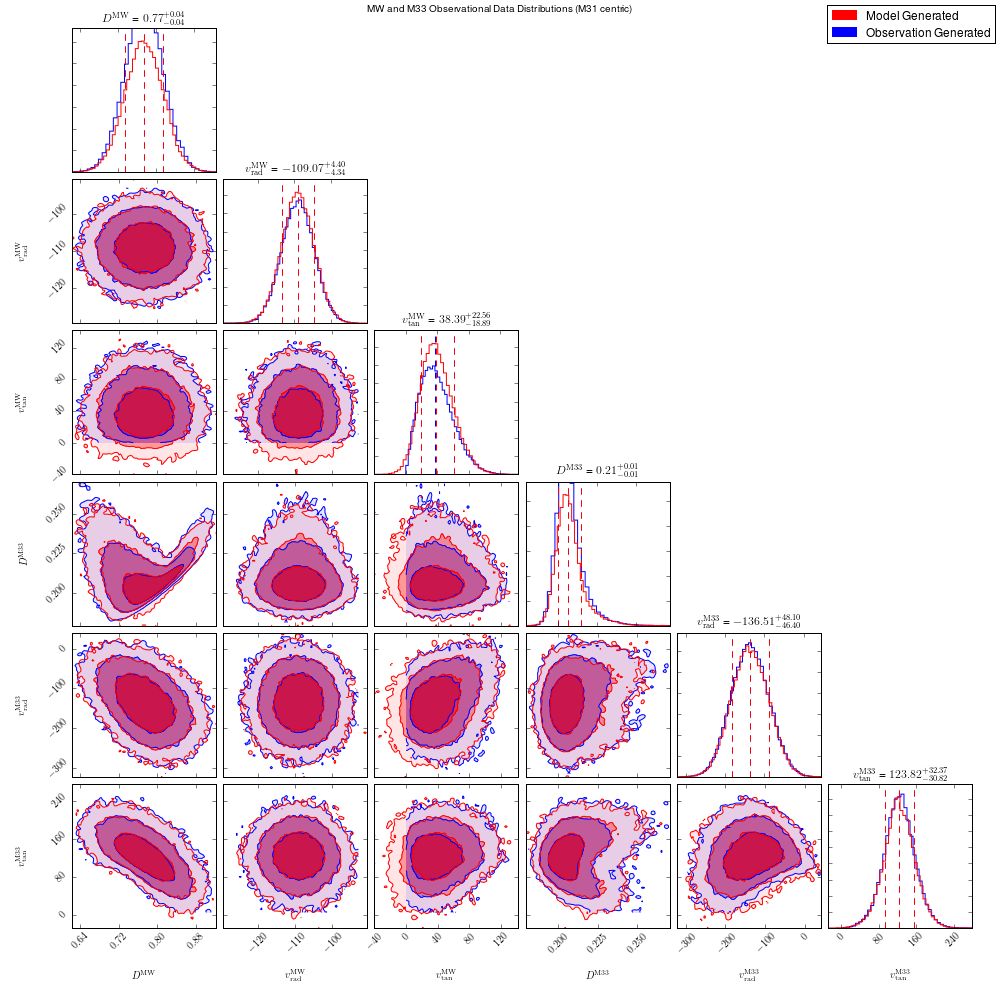
\includegraphics[width=\textwidth]{plots/model_gof.png}
  \caption{The 1-D and 2-D marginalizations of the parameter space used to create the GMM model. The sample generated from the observed values of the 6 parameters (blue) and the sample drawn from the resulting GMM (red) overlap almost perfectly.}
  \label{fig:gof}
\end{figure*}

\begin{figure*}
  \centering 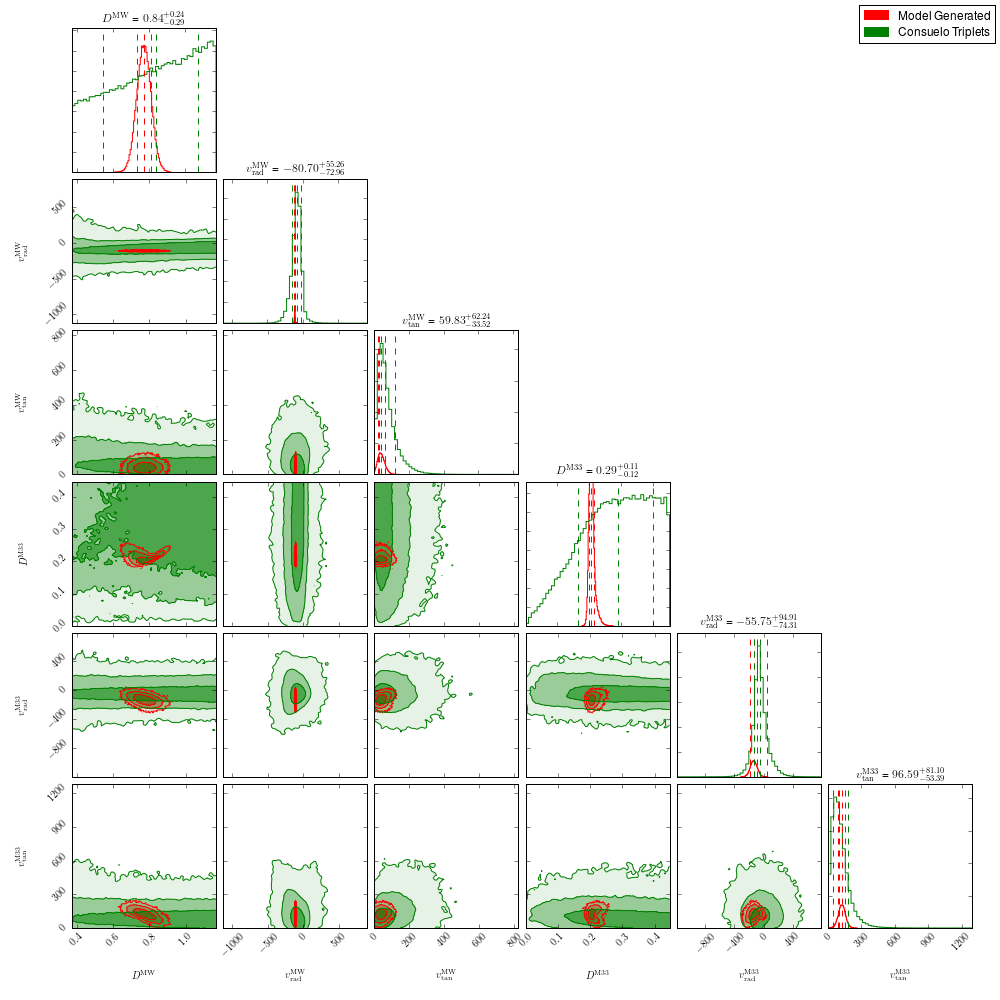
\includegraphics[width=\textwidth]{plots/sim_plot.png}
  \caption{The 1-D and 2-D marginalizations of the CONSUELO triplet sample (green) overlayed with the corresponding marginalizations from the sample drawn from the GMM model (red). The intersection shows which of the CONSUELO triplets are given the most weight by the model.}
  \label{fig:sim_plot}
\end{figure*}

% ----------------------------------------------------------------------------

\section{Results}
\label{sec:results}

% - - - - - - - - - - - - - - - - - - - - - - - - - - - - - - - - - - - - - - 

\subsection{The Mass of the Local Group from the Kinematics of M31}
\label{sec:results:LGmass}

Pairs: D, vr, vt constraints from M31. 
Measurement of  MLG. Precision. 

Figure: 1D plot of Pr(MLG) given \\
  1) M31 distance\\
  2) M31 vr\\
  3) M31 vt\\
  4) M31 all kinematics

Corner plot of Pr(MMW, MM31, MLG), prior vs all constraints

\begin{figure}
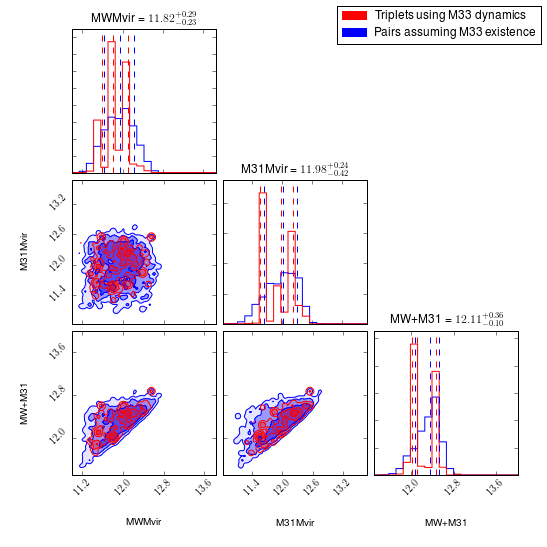
\includegraphics[width=\linewidth]{plots/res_plot.png}
  \caption{Log masses (units of $M_{\odot}$) of the MW, M31, and the LG weighted by likelihood. The displayed values above the histograms are the triplet numbers.}
  \label{fig:res_plot}
\end{figure}

\begin{figure}
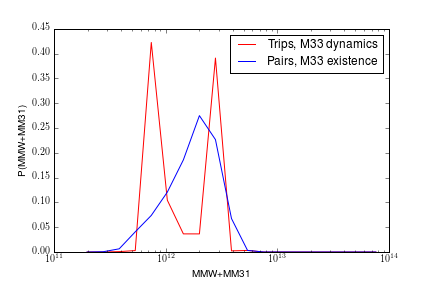
\includegraphics[width=\linewidth]{plots/pdf_lg_plot.png}
  \caption{The likelihood distribution of the mass of the Local Group. The Triplet distribution suffers from small statistics.}
  \label{fig:lg_pdf}
\end{figure}

\begin{figure}
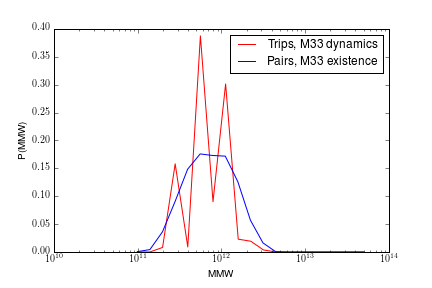
\includegraphics[width=\linewidth]{plots/pdf_mw_plot.png}
  \caption{The likelihood distribution of the mass of the MW. The Triplet distribution suffers from small statistics.}
  \label{fig:mw_pdf}
\end{figure}

% - - - - - - - - - - - - - - - - - - - - - - - - - - - - - - - - - - - - - - 

\subsection{The Mass of M31 from the Kinematics of M33}
\label{sec:results:M31mass}

Couples: D, vr, vt constraints from M33 given an M31-MW pair. 
Measurement of  MM31. Precision. 

Figure: 1D plot of Pr(MM31) given \\
  1) M33 distance\\
  2) M33 vr\\
  3) M33 vt\\
  4) M33 all kinematics

Corner plot of Pr(MM31, MM33, Mcouple), prior vs all constraints

% - - - - - - - - - - - - - - - - - - - - - - - - - - - - - - - - - - - - - - 

\subsection{The Masses of the Local Group Galaxy Halos from the Kinematics of M31 and M33}
\label{sec:results:jointanalysis}

Triplets: D, vr, vt constraints from M33 and M31. 
Measurement of MMW. Precision. 

Figure: 1D plot of Pr(MMW) given \\
  1) M31 kinematics\\
  2) + M33 kinematics\\

Figure: Corner plot of Pr(MMW, MM31, MM33, MLG) given\\
   1) prior \\
   2) all kinematics \\

% - - - - - - - - - - - - - - - - - - - - - - - - - - - - - - - - - - - - - - 

\subsection{Comparison with the Local Group Timing Argument Mass Estimate}
\label{sec:results:TA}

Timing argument introduction. Review of Li \& White. Two halo sum, M31
kinematics, "radial" MTA. Review of VdM12's comment on precision - aim is to
update Li\&White, show improvement in precision.  

Can compute radial MTA for every model local group,  and compare with actual
sums of M200. "Calibration" in sense that MTA gives estimate of MW + M31
masses, under assumption they are point masses on Keplerian orbits. Bias and
scatter both important.

Figure: corner plot of MLG, MTA, A200 given \\
  1) M31 kinematics (pairs+DvrM31)\\
  2) M31 + M33 kinematics (triplets+DVrM31+DVrM33)\\

% - - - - - - - - - - - - - - - - - - - - - - - - - - - - - - - - - - - - - - 

\subsection{Focusing on the Milky Way: constraints from other M31 and M33 halo mass estimates}
\label{sec:results:MW}

Review other measurements of M31 and M33 halos. Adopt one, possibly from
VdM12. Plot impact on Pr(MMW, MM31, MM33, MLG) and MW mass estimate. MW mass
estimate, precision. Tension?

Figure: Corner plot of Pr(MMW, MM31, MM33, MLG) given\\
   1) M31 and M33 kinematics (from earlier) \\
   2) these plus M31 and M33 halo mass estimates. \\

% - - - - - - - - - - - - - - - - - - - - - - - - - - - - - - - - - - - - - - 

%%%%%%%%%%%%%%%%%%%%%%
% \begin{deluxetable*}{lccccccc}
\tabletypesize{\small}
\tablecaption{\label{tab:masses}
Local group mass estimates}
\tabletypesize{\small}
\arraystretch{1.2}
\tablehead{
Constraints & 
$\log_{10} M_{\rm MW} / M_{\odot}$       & 
$\log_{10} M_{\rm M31} / M_{\odot}$      & 
$\log_{10} M_{\rm M31} / M_{\rm MW}$     & 
$\log_{10} M_{\rm M33} / M_{\rm MW}$     & 
$\log_{10} M\prime_{\rm LG} / M_{\odot}$ & 
$\log_{10} M_{\rm TA} / M_{\odot}$       & 
$\log_{10} A_{200}$ \\} 
\startdata
Pairs                &  $ 11.70^{+0.62}_{-0.41} $  &  $ 11.61^{+0.61}_{-0.48} $  &  $ -0.16^{+0.51}_{-0.59} $       &  --                         &  $ 12.02^{+0.65}_{-0.39} $  &  $ 9.4^{+3.1}_{-0.0} $  &   $ -1.95^{+1.90}_{-0.63} $ \\
$+$ M31 $D,v$        &  $ 12.33^{+0.41}_{-0.53} $  &  $ 12.24^{+0.40}_{-0.52} $  &  $ -0.08^{+0.75}_{-0.85} $       &  --                         &  $ 12.72^{+0.23}_{-0.27} $  &  $ 12.709^{+0.045}_{-0.051} $  &   $ -0.04^{+0.27}_{-0.19} $ \\
$+$ Bolshoi MW mass  &  $ 12.156^{+0.099}_{-0.087} $  &  $ 12.46^{+0.29}_{-0.49} $  &  $ 0.24^{+0.36}_{-0.46} $     &  --                         &  $ 12.65^{+0.20}_{-0.26} $  &  $ 12.706^{+0.044}_{-0.051} $  &   $ 0.03^{+0.26}_{-0.20} $ \\
Triplets             &  $ 11.74^{+0.52}_{-0.31} $  &  $ 11.99^{+0.48}_{-0.43} $  &  $ 0.12^{+0.55}_{-0.48} $        &  $ 11.26^{+0.24}_{-0.21} $  &  $ 12.28^{+0.41}_{-0.36} $  &  $ 12.04^{+0.52}_{-2.62} $  &   $ -0.35^{+0.32}_{-2.38} $ \\
$+$ M31 $D,v$        &  $ 12.10^{+0.43}_{-0.49} $  &  $ 12.50^{+0.23}_{-0.50} $  &  $ 0.31^{+0.69}_{-0.69} $        &  $ 11.28^{+0.37}_{-0.22} $  &  $ 12.71^{+0.12}_{-0.22} $  &  $ 12.698^{+0.058}_{-0.045} $  &   $ -0.02^{+0.23}_{-0.11} $ \\
$+$ M33 $D,v$        &  $ 12.30^{+0.35}_{-0.45} $  &  $ 12.48^{+0.19}_{-0.48} $  &  $ 0.13^{+0.72}_{-0.89} $        &  $ 11.40^{+0.39}_{-0.24} $  &  $ 12.781^{+0.052}_{-0.086} $  &  $ 12.725^{+0.030}_{-0.042} $  &   $ -0.077^{+0.102}_{-0.017} $ \\
$+$ Bolshoi MW mass  &  $ 12.048^{+0.156}_{-0.012} $  &  $ 12.660^{+0.046}_{-0.255} $  &  $ 0.54^{+0.11}_{-0.30} $  &  $ 11.66^{+0.26}_{-0.39} $  &  $ 12.773^{+0.016}_{-0.160} $  &  $ 12.724^{+0.019}_{-0.076} $  &   $ -0.06^{+0.18}_{-0.00} $ \\
\enddata
\tablecomments{}
\end{deluxetable*}

%%%%%%%%%%%%%%%%%%%%%%

% ----------------------------------------------------------------------------

\section{Discussion}
\label{sec:discuss}


% \subsection{Statistical Robustness}
% \label{sec:bootstrap}
% 
% \subsection{The Information Content of the Observations}
% \label{sec:bootstrap}
% Improvements in measurements from cosmological prior? eg distances?
% 
% 
% \subsection{The Masses of M31 and M33: Comparison with Stellar Dynamics
% Results}
% \label{sec:M31M33stellardynamics}
% 
% 
% \subsection{The Local Group Mass: Comparison with the Timing Argument}
% \label{sec:timing}
% 
% 
% \subsection{Further Work}
% \label{sec:future}
% 
% ----------------------------------------------------------------------------

\section{Conclusions}
\label{sec:conclude}

From this analysis we draw the following conclusions:
\begin{itemize}

\item The \consuelo simulation has sufficient volume to permit analogs of
individual galaxy groups to be identified in large numbers. We identified XX
3-member groups with similar isolation properties to the Local Group.

\item Importance-sampling the \consuelo-sampled halo parameter prior PDF with
the probability of the M31 and M33 distances and velocities, and the mass of
the Milky Way, we infer a two-halo Local Group mass of $\MLG = (\MMW + \MEI)
= (\MPAIRestimate^{+\MPAIRerrorplus}_{-\MPAIRerrorminus}) \times 10^{12}
\Msun$.

\item M31-MW timing mass argument superceded. How accurate was it? 

\item Weighed M31 using M33 kinematic information. Result.

\item Combining M31 and M33 kinematics to weigh halos. Inferences of the three
halo masses. MW mass. Tension with other datasets?

% \item We find that the M33 halo provides a significant addition to the Local
% Group mass: $\MEE = (\MEEestimate^{+\MEEerrorplus}_{-\MEEerrorminus}) \times
% 10^{12} \Msun$. Including the M33 halo increases the inferred Local Group mass
% to $\MTRIPLET = (\MMW + \MEI + \MEE) =
% (\MTRIPLETestimate^{+\MTRIPLETerrorplus}_{-\MTRIPLETerrorminus}) \times
% 10^{12} \Msun$. We infer the mass of M31 to be $\MEI =
% (\MEIestimate^{+\MEIerrorplus}_{-\MEIerrorminus}) \times 10^{12} \Msun$
% 
% \item For each sample Local Group analog, we can compute the timing argument
% mass that an observer at the Earth analog's position would derive: the PDF for
% this quantity is ... relative to that for the true Local Group mass. We find
% that ... 
% 
% \item The M33 kinematics contain information about the proper motion of M31:
% we predict this to be...

\end{itemize}

% ----------------------------------------------------------------------------
%\nocite{*}
%\bibliographystyle{unsrt}
%\bibliography{references.bib}



% ----------------------------------------------------------------------------
\nocite{*}
\bibliography{references}

\end{document}

